\renewcommand{\BrainFuckChapter}{%
  {+}{+}{+}{+}{+}{+}{+}{+}{[}{>}{+}{+}{+}{+}{>}{+}{+}{+}{+}{+}{+}{>}{+}{+}{+}{+}{+}{+}{+}{+}{>}{+}{+}{+}{+}{+}{+}{+}{+}{+}{+}{>}{+}{+}{+}{+}{+}{+}{+}{+}{+}{+}{+}{+}{<}{<}{<}{<}{<}{-}{]}{>}{>}{>}{>}{-}{-}{-}{.}{-}
  {-}{-}{-}{-}{.}{+}{+}{+}{+}{+}{+}{+}{+}{+}{+}{+}{.}{<}{<}{+}{+}{.}{<}{.}{>}{-}{-}{-}{-}{-}{.}{<}{.}{>}{>}{>}{-}{-}{-}{.}{>}{+}{.}{+}{+}{+}{+}{+}{+}{+}{+}{+}{+}{+}{+}{+}{+}{+}{+}{+}{.}{<}{+}{+}{+}{+}{+}{+}{+}{+}
  {+}{+}{+}{+}{+}{+}{+}{+}{+}{.}{>}{-}{-}{-}{-}{-}{-}{.}{.}{<}{+}{+}{+}{+}{.}{>}{.}{-}{-}{-}{.}{+}{+}{+}{+}{+}{+}{+}{+}{+}{+}{+}{+}{+}{+}{+}{+}{+}{.}{<}{-}{-}{-}{-}{.}{>}{-}{-}{-}{-}{-}{-}{.}{<}{+}{+}{+}{+}{+}{+}
  {+}{+}{.}{>}{-}{-}{-}{-}{-}{.}{-}{.}{[}{>}{]}{<}{[}{[}{-}{]}{<}{]}{+}{-}{>}{-}{>}{-}{>}{-}{<}{>}{-}{-}{>}{>}{>}{+}{>}{>}{-}{+}{<}{>}{-}{>}{+}{+}{+}{-}{>}{>}{-}{+}{-}{>}{>}{>}{<}{>}{<}{<}{<}{>}{+}{<}{<}{<}{>}{<}
}
\renewcommand{\LifeChapter}{y}

\newcommand{\strideFn}{\emph{Stride}}
\newcommand{\randomFn}{\emph{Random}}
\newcommand{\nproc}{\mathit{np}}

\chapter{\mhsII{} -- Parallelization}
\label{sec:mhs2p}
In this section we present the parallelized version of \ac{MHSII}.
%
As explained in
\CrefPageParen{sec:intro:research-goals:horizontal-scalability}, our
goal in this chapter is to enable the computation of \acp{MHS} in
parallel or even distributed environments.


This chapter is divided as follows.
%
First, we introduce our \ac{MHS} generation algorithm.
%
Second, we evaluate the performance of our algorithm.

\section{Approach}
\label{sec:mhs2p:approach}
The parallel algorithm can be seen as a Map-Reduce algorithm
\citep{Dean04} (\Cref{fig:mhs2p:map-reduce}).
%
The map task (\Cref{alg:mhs2p:map}) is a modified version of
\CrefPageParen{alg:mhs2o}.

\begin{figure}[!ht]
  \includegraphics[page=5]{figures/mhs2/figures/parallel/main}
  \caption{\acs{MHSII} Map-Reduce workflow\label{fig:mhs2p:map-reduce}}
\end{figure}



\begin{algorithm*}
  \begin{description}
  \item[Inputs:]\ $(U, S, d=\emptyset, D=\emptyset)$
  \item[\ColorLine Parameters:]\ $(L,\fn{Skip}, k, \nproc)$
  \item[Output:]\ Minimal hitting set collection $D'_k$
  \end{description}

  \begin{algorithmic}[1]
    \If{$\exists_{s \in S} : s \cap U = \emptyset$} \label{alg:mhs2p:map:opt3}
    \State \Return $D$
    \EndIf
    \If{$S \not= \emptyset$} \label{alg:mhs2p:map:divide}
    \State $U \gets U \setminus \set{j \mid j \in U \wedge (\nexists_{s \in S}: j\in s)}$ \label{alg:mhs2p:map:opt2}
    \For{$j \in  \fn{Rank}(U, S)$} \label{alg:mhs2p:map:rank}
    \CIF{$|d| + 1 = L \wedge \fn{Skip}(k,\nproc)$} \label{alg:mhs2p:map:skip}
    \CSTATE $U \gets U \setminus \set{j}$   \algorithmiccomment{\Opt{1}} \label{alg:mhs2p:map:opt1.1}
    \CSTATE \textbf{continue}
    \EndIf
    \State $S' \gets \set{s \mid s \in S \wedge j \in s}$ \label{alg:mhs2p:map:S'}
    \State $U \gets U \setminus \set{j}$  \label{alg:mhs2p:map:opt1.2}
    \State $D \gets \fn{MHS^\text{\smaller2}}(U  \setminus \set{j}, S \setminus S', d \cup \{j\}, D)$
    \EndFor
    \Else
    \If{$\nexists_{d'\in D}: d'\subseteq d$} \label{alg:mhs2p:map:isminimal}
    \State $D \gets D \setminus \{d' \mid d' \in D \wedge  d \subseteq d'\}$ \label{alg:mhs2p:map:purge}
    \State $D \gets D \cup \{d\}$ \label{alg:mhs2p:map:addD}
    \EndIf
    \EndIf
    \State \Return $D$
  \end{algorithmic}
  \caption{\acs{MHSII} -- Map task\label{alg:mhs2p:map}}
\end{algorithm*}

In contrast to the sequential algorithm, we added a parameter $L$ that
sets the \textit{fork-level}, \ie, the number of calls in the stack
(or equivalently, $|d| + 1$), at which the computation is divided
among the processes/threads.
%
When a process of the distributed algorithm reaches the target level
$L$, it uses a load division function ($\fn{Skip}$) to decide which
elements of the ranking to skip or to analyze.
%
The value of $L$ implicitly controls the granularity of decision of
the load division function at the cost of performing more redundant
calculations (\Cref{fig:mhs2p:L-param}).
%
Implicitly, by setting a value $L > 1$, all processes redundantly
compute all \ac{HS} such that $|d| < L$.
\begin{figure}[ht!]
  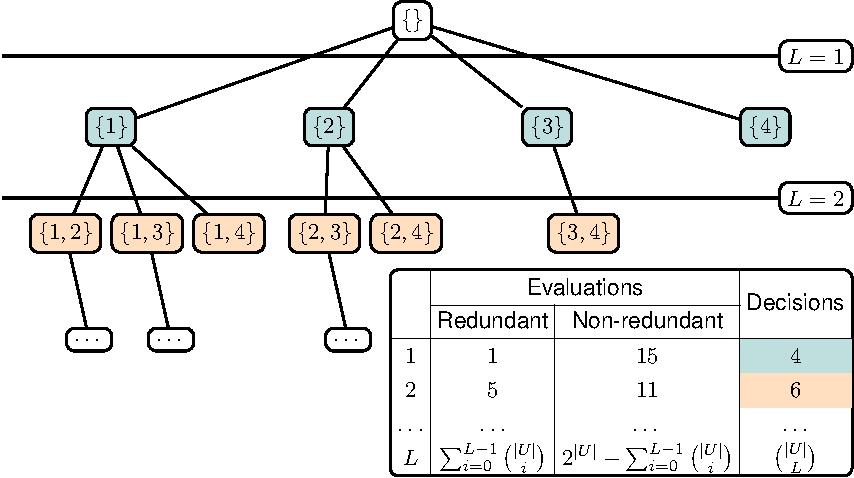
\includegraphics[page=1]{figures/mhs2/figures/parallel/main}
  \caption{$L$ parameter intuition\label{fig:mhs2p:L-param}}
\end{figure}

In parallel processing environments, it is desirable to minimize the amount of time processes are idle.
%
Idleness periods may arise when a process completes its work before
other threads on which subsequent processing stages depend on.
%
Concretely, for Map-Reduce algorithms, it is desirable that all map
complete their jobs simultaneously, thus minimizing idle periods and
improving resources usage.
%
Taking this fact into account, a correct selection of the load
distribution function (\ie,$\fn{Skip}$) is critical for obtaining good
performance.
%

With regard to the load division, we propose two different approaches.
%
The first, referred to as \strideFn{}, consists in assigning elements
of the ranking to processes cyclically
(\Cref{fig:mhs2p:skip-fn-stride}).
%
Formally, a process $p_{k \in\set{1..\nproc}}$ is assigned to a branch
$b_l$ of the search tree if:
\begin{equation}
  l \mod{\nproc} = k - 1
\end{equation}
%

The second approach, referred to as \randomFn{}, uses a
pseudo-random generator to divide the computation (\Cref{fig:mhs2p:skip-fn-random}).
%
This random generator is fed into a uniform distribution generator
that assures that, over time, all $p_k$ get assigned a similar number
of elements although in random order.
%
This method is aimed at obtaining a more even distribution of the
problem across processes than \strideFn{}
(\Cref{fig:mhs2p:stride-balancing}).
%
Formally, a process $p_{k \in\set{1..\nproc}}$ is assigned to an element of
the ranking if:
\begin{equation}
  \fn{rand}() \mod{\nproc} = k - 1
\end{equation}
%
A particularity of this approach is that the seed of the pseudo random
generator must be shared across every process to assure that no
further communication is needed.
\begin{figure}[!ht]
  \tikzstyle{p1}=[inner sep=0.1em, draw=black, circle, fill=blue!30!white]
  \tikzstyle{p2}=[inner sep=0.1em, draw=black, circle, fill=yellow!30!white]
  \begin{subfigure}{0.48\columnwidth}
    \centering
    \includegraphics[page=2]{figures/mhs2/figures/parallel/main}
    \caption{\strideFn{} function\label{fig:mhs2p:skip-fn-stride}}
  \end{subfigure}
  \hfill{}
  \begin{subfigure}{0.48\columnwidth}
    \centering
    \includegraphics[page=3]{figures/mhs2/figures/parallel/main}
    \caption{\randomFn{} function\label{fig:mhs2p:skip-fn-random}}
  \end{subfigure}
  \caption{$\fn{Skip}$ functions intuition\label{fig:mhs2p:skip-fn}}

\end{figure}

\begin{figure}[!ht]
  \includegraphics[page=4]{figures/mhs2/figures/parallel/main}
  \caption{Balancing problem when using the \strideFn{} function\label{fig:mhs2p:stride-balancing}}
\end{figure}


\begin{algorithm*}
  \begin{description}
  \item[Inputs:]\ $(D'_1, ..., D'_{\nproc})$
  \item[Output:]\ Minimal hitting set collection $D$
  \end{description}
  \begin{algorithmic}[1]
    \State $D \gets \emptyset$
    \State $D' \gets \fn{Sort}(\bigcup^{\nproc}_{k=1} D'_k)$
    \For{$d \in D'$}
    \If{$\nexists_{d'\in D}: d'\subseteq d$}\label{alg:reduce:isminimal}
    \State $D \gets D \cup \{d\}$
    \EndIf
    \EndFor
    \State \Return $D$
  \end{algorithmic}
  \caption{\acs{MHSII} -- Reduce task}
  \label{alg:mhs2p:reduce}
\end{algorithm*}


Finally, the reduce task (\Cref{alg:mhs2p:reduce}), responsible for
merging all partial \ac{MHS} collections $D'_{k\in\set{1..\nproc}}$
originating from the map task.
%
The reducer works by merging all \acp{HS} in a list, ordered by
cardinality.
%
The ordered list is then iterated, adding all \acp{MHS} to $D$.
%
As the \acp{HS} are inserted in an increasing cardinality order, it is
not necessary to look for subsumable \acp{HS} (line
\ref{alg:mhs2p:map:purge} in \Cref{alg:mhs2p:map}) in $D$, thus
improving the algorithm's performance.
\section{Benchmark}
\label{sec:mhs2p:results}
To assess the performance of our algorithm we conducted a set of
benchmarks in a setup similar to the one presented in
\CrefPageParen{sec:mhs2o:results}.
%
To evaluate the gains introduced by the parallelization of the
candidate generation algorithm we use the \emph{speedup} metric.
%
In parallel computing, speedup refers to how much a parallel algorithm
optimizes an arbitrary metric in relation to the corresponding
sequential algorithm.
%
Concretely, the speedup metric is defined as:
\begin{equation}
  S_p = \frac{M_1}{M_p}
\end{equation}
where:
\begin{itemize}
\item $p$ is the number of processors;
\item $M_1$ is the value of an arbitrary metric for the sequential
  algorithm;
\item $M_p$ is the value of the same arbitrary metric for the parallel
  algorithm with $p$ processors.
\end{itemize}

In small problems where \emph{all} minimal candidates are calculable,
the observed metric is the execution time, evaluating how much faster
is the parallel version of the algorithm when compared to its
sequential counterpart.
%
In large problems where only a subset of the solution is calculable,
we evaluate the algorithm's throughput improvement by registering the
number of minimal candidates calculated by the parallel algorithm with
different number of processors and constrained by the same calculation
time.

A normalized version of the speedup is called \emph{efficiency} and is
defined as:
\begin{equation}
  E_p = \frac{S_p}{p} = \frac{M_1}{p \times M_p}
\end{equation}

The efficiency value typically ranges between zero and one and
estimates how well-utilized the processors are in solving the problem,
compared to how much effort is wasted in communication and
synchronization.


\subsection{Small Problems}
\label{sec:mhs2p:results:small}

The first parallelization benchmark, is aimed at evaluating the
behavior of \ac{MHSII} for small problems ($M = N = 40$, $R \in
\{0.25,0.5,0.75\}$).


\begin{figure}[!ht]
  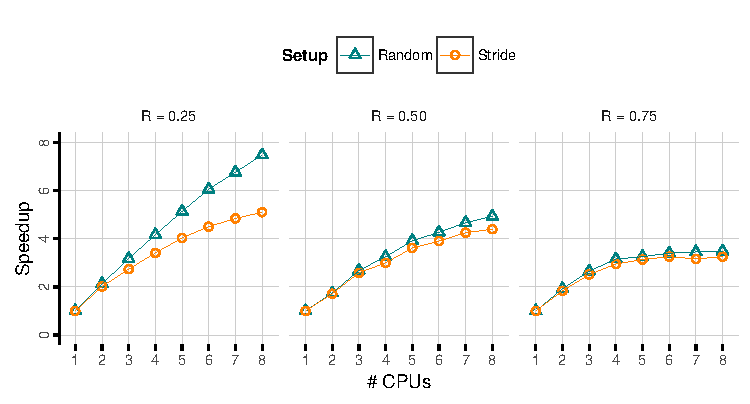
\includegraphics[trim=0.5em 2.65em 0em 0em, clip,
  page=1]{figures/mhs2/figures/parallel_small.pdf}
  \\[0.5em]
  \includegraphics[trim=0.5em 2.65em 0em 5.5em, clip, page=2]{figures/mhs2/figures/parallel_small.pdf}
  \\[0.5em]
  \includegraphics[trim=0.5em 2.65em 0em 5.5em, clip, page=4]{figures/mhs2/figures/parallel_small.pdf}
  \\[0.5em]
  \includegraphics[trim=0.5em 0em 0em 5.5em, clip, page=3]{figures/mhs2/figures/parallel_small.pdf}
  \caption{Small problems' results\label{fig:mhs2p:results:small}}

\end{figure}

In \Cref{fig:mhs2p:results:small}, we plot the speedup as well as the
efficiency for both the \strideFn{} and \randomFn{} load distribution
functions.
%
Also, \Cref{fig:mhs2p:results:small} shows the run-times\footnote{In
  this plot, each cluster is composed of $1$ data point per test case
  (100 data points for each load distribution function). The
  horizontal displacement inside each cluster was only added to
  improve the visualization of the results.} as well as the
throughput\footnote{In this section the throughput represents the
  average throughput per thread.
  %
  Concretely it is calculated as $\displaystyle\frac{|D|}{\nproc
    \times t}$, where $t$ represents the cut-off time.} for both load
distribution functions.

The analysis of \Cref{fig:mhs2p:results:small} shows different
speedup/efficiency patterns for different $R$ values, which are due to
the large variation in the run times: $\approx 200$, $5.7$ and $0.1$
seconds for $R=\{0.25,0.5,0.75\}$, respectively.
%
On the one hand, when the run time is small (\ie, for large $R$
values), the parallelization overhead has a higher relative impact in
the algorithm's performance.
%
On the other hand, when the run time becomes larger due to the
increase of both the cardinality and the amount of \acp{MHS} (\ie, for
small $R$ values), the relative parallelization overhead becomes
almost insignificant.


For $R = 0.25$ and in contrast to $R \in \{0.5,0.75\}$, the
speedup/efficiency of \randomFn{} is superior to the performance
of \strideFn{}.
%
The reason for such a difference in efficiency is that the
\emph{cool-down period} (\ie, the period in which at least one process
is idle and another is active) of \strideFn{} was longer than the one
observed for \randomFn{}.
%
The smaller \emph{cool-down} period of \randomFn{} shows that the
usage of a stochastic approach was successful at evenly dividing an
unbalanced search tree among threads, leading to a better load
division.

Finally, we observe that \randomFn{} experienced \emph{super-linear}
speedup (i.e, efficiency above 100\%) for some of the test
cases.
%
This pattern emerges due to the fact that the complexity of the
operations performed on $D$ (lines \ref{alg:mhs2p:map:isminimal} --
\ref{alg:mhs2p:map:addD} in \Cref{alg:mhs2p:map}), is not linear in
the number of elements stored in it.
%
As a consequence, by reducing size of $D$ to $\frac{1}{\nproc}$ %$
effectively reduces the cost of the operations by a factor greater than
$\nproc$.
\FloatBarrier
\subsection{Large Problems}
\label{sec:mhs2p:results:large}

The second benchmark is aimed at evaluating the behavior of \ac{MHSII}
for large problems ($M = N = 10^3$, and $R \in \{0.25,0.5,0.75\}$).

\begin{figure}[!ht]
  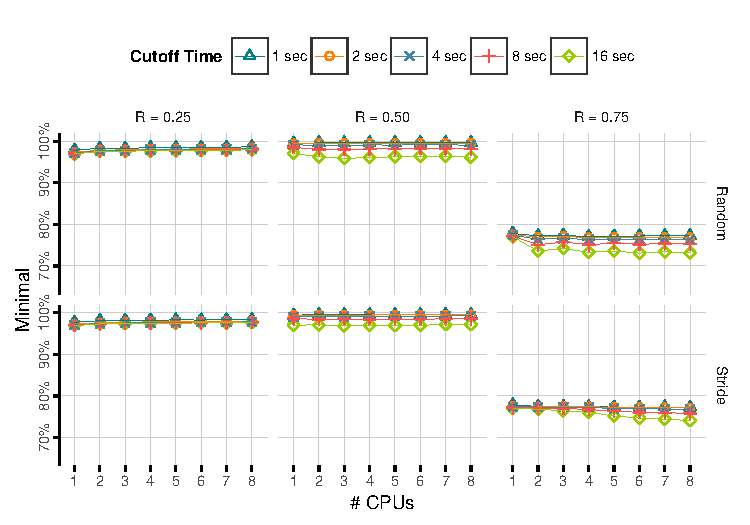
\includegraphics[trim=0.5em 2.65em 0em 0em, clip, page=1]{figures/mhs2/figures/parallel_large.pdf}
  \\[0.5em]
  \includegraphics[trim=0.5em 0em 0em 5.5em, clip, page=6]{figures/mhs2/figures/parallel_large.pdf}
  \caption{Large problems' results\label{fig:mhs2p:results:large}}
\end{figure}

\Cref{fig:mhs2p:results:large} shows the minimality percentage and
throughput for the large problems when using time-based cutoffs of $1,
2, 4, 8,$ and $16$ seconds per process with a varying number of
processes.

It appears that, for large problems, there is no significant
difference in terms of the amount of generated \acp{MHS} between
\randomFn{} and \strideFn{}.
%
By performing a two-tailed T-test we determined, with a $99\%$
confidence interval, that both approaches should have, on average,
equal throughputs.
%

Regarding the minimality percentage of both approaches, we observed
similar results to those presented in
\CrefPageParen{fig:mhs2o:results:large}: $97\%$ for $R =
\{0.25,0.5\}$, while for $R=0.75$ the percentage decreases to around
$75\%$.
%
Also, the throughput is consistent with all previous benchmarks.

\begin{figure}[ht]
  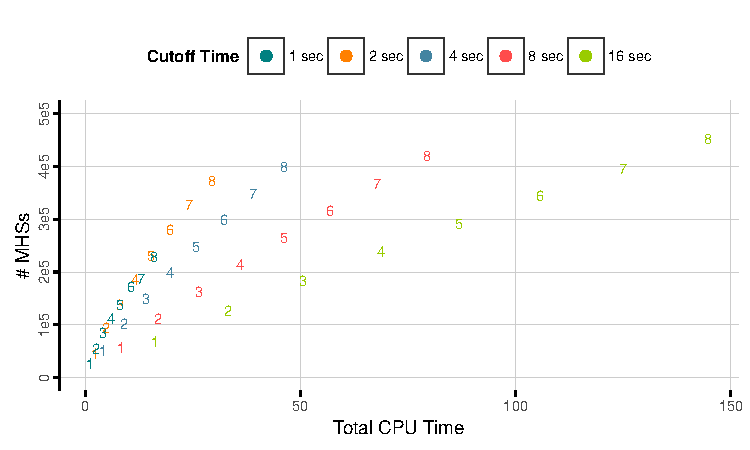
\includegraphics[trim=0.5em 2.65em 0em 0em, clip, page=1]{figures/mhs2/figures/parallel_scatter_large.pdf}
  \includegraphics[trim=0.5em 0em 0em 3.3em, clip, page=3]{figures/mhs2/figures/parallel_scatter_large.pdf}
  \caption{Large problems' results with x-axis
    transformation\label{fig:mhs2p:results:large-scatter-linear}}
\end{figure}

\Cref{fig:mhs2p:results:large-scatter-linear} shows the number of
\acp{MHS} and throughput after applying a data transformation.
%
In spite of using the number of processes as the x-axis, we use the
total \ac{CPU} time for all processes ($rt_{cpu}$), which is
calculated as:
\begin{equation}
  rt_{cpu} = rt_{wall} \times \nproc
\end{equation}
where $rt_{wall}$ is the perceived run time for the algorithm's
execution when using a ``wall'' clock%
\footnote{Since $rt_{wall}$ accounts for both the map and reduce
  phases whereas the cutoff is only applied to the map phase, it is
  always larger than the cutoff value.}.
%
Each data point is represented by a number encoding the number of used
\acp{CPU}%
\footnote{The points' y-axis values are the averages over the
  different $R$ values for the data points in
  \Cref{fig:mhs2p:results:large}.}.
%
We can see that, for instance, running the algorithm for $8$ seconds
on $8$ \acp{CPU} accounts approximately for the same total run-time as
running the algorithm for $16$ seconds on $4$ \acp{CPU}.


Using this plot we can easily see that, for a given total calculation
time, it is, on average, preferable to divide the task among the
maximum possible number of \acp{CPU} (eventually, given enough
\acp{CPU}, this trend should hit a ceiling).
%
As an example, we can see that $8$ threads running for $2$ seconds
produce more \acp{MHS} than $2$ threads running for $16$ despite using
approximately the same total \ac{CPU} time.
%
This result is in accordance with the super-linear
speedup observed in \Cref{fig:mhs2p:results:small}.

\section{Summary}
In this chapter we successfully addressed the limitations presented in
\CrefPageParen{sec:intro:research-goals:horizontal-scalability}
thereby positively answering \CrefPageParen{rq:scalability}.
%
Concretely, in this chapter:

\begin{itemize}[nolistsep]
\item We proposed a parallelization approach for \ac{MHSII}
  (\CrefPageSee[]{sec:mhs2p:approach}):
  \begin{itemize}
  \item We proposed an approach based on the Map-Reduce paradigm,
    thereby being applicable in both parallel and distributed
    environments.
  \item We proposed two load distribution strategies: \strideFn{} and
    \randomFn{}.
  \end{itemize}

\item We presented the conducted benchmarks showing that:
  \begin{enumerate}
  \item When computing full solutions for complex enough problems, the
    algorithm performs at approximately $100\%$ efficiency even when
    using $8$ worker threads
    (\CrefPageSee[]{sec:mhs2p:results:small}).
  \item When solving simple problems for which the algorithm's
    run-time is small, the efficiency quickly drops with the increase
    of worker threads (\CrefPageSee{sec:mhs2p:results:small}).
  \item On average, the algorithm was more efficient when the problem
    was divided across the maximum number of threads
    (\CrefPageSee{sec:mhs2p:results:large}).
  \item The algorithm exhibits a similar throughput per thread in both
    small/large problems and sequential/parallel setups
    (\Cref{fig:mhs2o:results:small,fig:mhs2o:results:large,fig:mhs2p:results:small,fig:mhs2p:results:large},
    pages \pageref{fig:mhs2o:results:small},
    \pageref{fig:mhs2o:results:large},
    \pageref{fig:mhs2p:results:small} and
    \pageref{fig:mhs2p:results:large}, respectively).
  \end{enumerate}
\end{itemize}

The usage of parallel processing enables the exploration of a larger
number of \ac{HS}, increasing the likelihood of actually finding the
``best'' \ac{MHS} for a particular instance of the problem.
%
In the particular case of \ac{SFL}, and as stated in
\CrefPageParen{sec:mhs2o:summary}, this improvement translates into:
\begin{itemize}
\item Better diagnostic accuracy when setting a time-based cutoff,
  due to the fact that calculating more candidates increases the
  likelihood of finding the correct candidate.
\item Smaller diagnostic latency when setting a solution size cutoff,
  due to the fact that calculating a fixed amount of diagnostic
  candidates takes less time with \ac{MHSII} than with \staccato{}.
\end{itemize}
